\documentclass{article}

\usepackage{neurips_2019_author_response}

\usepackage[utf8]{inputenc} % allow utf-8 input
\usepackage[T1]{fontenc}    % use 8-bit T1 fonts
\usepackage{hyperref}       % hyperlinks
\usepackage{url}            % simple URL typesetting
\usepackage{booktabs}       % professional-quality tables
\usepackage{amsfonts}       % blackboard math symbols
\usepackage{nicefrac}       % compact symbols for 1/2, etc.
\usepackage{microtype}      % microtypography

\usepackage{lipsum}

\usepackage{epsfig}
\usepackage{graphicx}
\usepackage{amsmath}
\usepackage{amssymb}

\usepackage{mathrsfs}
\usepackage{datetime}

\usepackage{algorithm}% http://ctan.org/pkg/algorithm
\PassOptionsToPackage{noend}{algpseudocode}% comment out if want end's to show
\usepackage{algpseudocode}% http://ctan.org/pkg/algorithmicx

\makeatletter
\newcommand*{\skipnumber}[2][1]{%
   {\renewcommand*{\alglinenumber}[1]{}\State #2}%
   \addtocounter{ALG@line}{-#1}}
\renewcommand{\ALG@beginalgorithmic}{\small}
\makeatother

\usepackage{etoolbox}
% the following line injects our new indent handling code in place of the default spacing
% \patchcmd{\ALG@doentity}{\noindent\hskip\ALG@tlm}{\ALG@printindent}{}{\errmessage{failed to patch}}
% \makeatother
% end vertical rule patch for algorithmicx

\usepackage{tabularx}
\usepackage{lipsum}
\usepackage{makecell}
\renewcommand\theadfont{}
\usepackage{multirow}
\usepackage[labelformat=simple]{subcaption}
\renewcommand\thesubfigure{(\alph{subfigure})}
\usepackage{booktabs}
\usepackage{rotating}
\newcolumntype{?}{!{\vrule width 0.3em}}

\newcommand*{\cost}{w}%
\newcommand*{\interact}{\mathcal{W}}
\newcommand*{\algname}{GASP}
\newcolumntype{M}[1]{>{\centering\arraybackslash}m{#1}}


\DeclareMathOperator*{\argmax}{arg\,max}
\DeclareMathOperator*{\argmin}{arg\,min}
\usepackage{mathrsfs}
\newcommand{\RED}[1]{#1}

\newcommand\TODO[1]{{\color{red}{TODO: #1}}}
\newcommand\UPDATE[1]{{\color{blue}{#1}}}
\newcommand\SOURCE[1]{{\color{green}{(from: #1)}}}
% \newcommand\CHANGED[2]{{{\color{blue}{#1}}\color{green}{#2}}}

\usepackage[dvipsnames]{xcolor}
\usepackage[shortlabels]{enumitem}

\usepackage{amsthm}
\usepackage{thmtools,thm-restate}
\newtheorem{theorem}{Theorem}[section]
\newtheorem{prop}{Proposition}[section]

\usepackage{authblk}

\usepackage{etoolbox}
% \renewcommand\refname{}
\setlength{\bibsep}{2pt plus 5.4ex}


\begin{document}

\begin{figure}[t]
\captionsetup{font=small}
        \centering
\begin{minipage}[b]{0.38\textwidth}
\centering
        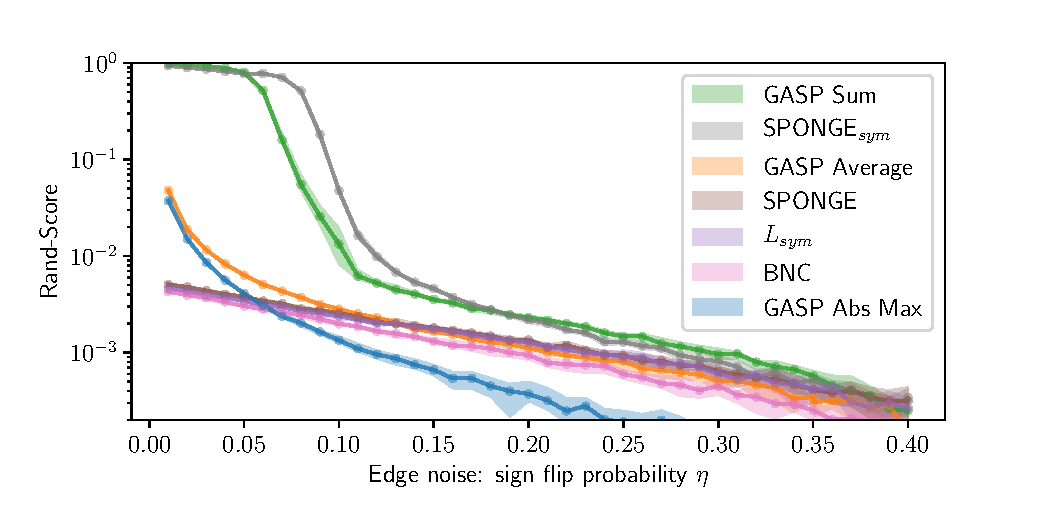
\includegraphics[width=\textwidth,trim=0.25in 0.25in 0.68in 0.36in,clip]{./SSBM_experiments.pdf}
        \captionof{figure}{Experiments on SSBM synthetic graphs}
    \label{fig:SSBM_experiments}
\end{minipage}\hfill
\begin{minipage}[b]{0.25\textwidth}
\centering
    \scriptsize
\begin{tabular}{l|c}
           Method & Rand-Score \\ \midrule
           GASP Average & 0.8966 \\
GASP Sum & 0.8965 \\
GASP Abs Max & 0.8932 \\
SPONGE$_{sym}$ \cite{Cucuringu2019SPONGEAG} & 0.4389\\
$L_{sym}$ \cite{kunegis2010spectral} & 0.1931 \\
SPONGE \cite{Cucuringu2019SPONGEAG} & 0.0789 \\
BNC \cite{chiang2012scalable} & 0.0074 \\
        \end{tabular}
    \captionof{table}{Experiments on CREMI}
    \label{tab:cremi_experiments}
\end{minipage}\hfill
\begin{minipage}[b]{0.30\textwidth}
\centering
    \scriptsize
\begin{tabular}{l|cc}
           Method & AP  & AP 50\% \\ \midrule
           PANet \cite{liu2018path} & \textbf{31.8} & \textbf{57.1} \\
           \textbf{GMIS + \algname{} Avg} & 28.3 & 47.0 \\ 
           GMIS & 27.3 & 45.6 \\
           Mask R-CNN & 26.2 & 49.9 \\
           SGN \cite{liu2017sgn} & 25.0 & 44.9 \\
           DIN \cite{arnab2017pixelwise} & 20.0 & 38.8 \\
           DWS \cite{bai2017deep} & 19.4 & 35.3 \\
           % InstanceCut \cite{kirillov2017instancecut} & 13.0 & 27.9 \\
        \end{tabular}
    \captionof{table}{Scores on CityScapes \emph{test} set}
    \label{tab:cityscapes_test}
\end{minipage}
\end{figure}

We appreciate the very helpful comments by all reviewers and will address their concerns in the final version.

\textbf{Comparison with spectral clustering (R3)}: 
As kindly suggested by Reviewer 3, we include additional experiments comparing GASP with the spectral clustering methods proposed in \cite{Cucuringu2019SPONGEAG,chiang2012scalable,kunegis2010spectral}. 
Similarly to most of spectral clustering approaches, these methods need to previously specify the number $k$ of final clusters. %or use some additional heuristic criterion to determine $k$. 
On the other hand, in our article we focused on algorithms and tasks related to \emph{correlation clustering}, which has the goal of partitioning a signed graph when the true number of clusters is unknown. 
%\UPDATE{Comment from R3: optionally mention fusion-moves comparison for list of algorithms that are actually used in practice...?}
As suggested by R3, we then generated synthetic graphs from a signed stochastic block model (SSBM) where the true number of clusters is previously known. In the experiments, we used an Erd\H os-R\'enyi random graph model $\mathcal{G}(N,p)$ with $N=10^5$ vertices and edge probability $p=0.1$. Following the approach in \cite{Cucuringu2019SPONGEAG}, we partitioned the graph into $k=100$ equally-sized clusters, such that edges connecting vertices belonging to the same cluster (\UPDATE{different clusters}) had Gaussian distributed edge weights centered at $\mu=1$ ($\mu=$-$1$) and with standard deviation $0.1$. To model noise, we flipped the sign of each edge independently with probability $\eta$. Results are shown in Fig. \ref{fig:SSBM_experiments}.
At the same time, we would also like to argue that computer vision is currently one of the most important machine learning application domains, so a success on real data from that domain should count no less than success on synthetic / toy data.
Thus, we extended the comparison with spectral methods to the task of neuron segmentation. Since the spectral methods cannot scale to the full CREMI dataset, we considered a random tiny crop of 10x100x100 voxels resulting in a graph with $10^5$ vertices and~$\sim10^6$ edges. Scores are summarized in Table \ref{tab:cremi_experiments}.\\
%suggested by the reviewer that performed best in the recent comparison \cite{Cucuringu2019SPONGEAG}: one based on the Balanced Normalized Cut (BNC) \cite{chiang2012scalable}; another on the symmetrically normalized Signed Laplacian ($L_{sym}$) \cite{kunegis2010spectral}; SPONGE and SPONGE$_{sym}$ algorithms were recently proposed in \cite{Cucuringu2019SPONGEAG}.
We would like to stress that in these experiments we compared GASP with the strongest possible baseline, by giving the true number of GT clusters as an input to the spectral methods. Despite this, GASP significantly outperformed other methods on neuro-data and achieved comparable scores on the SSBM synthetic data. The specific design choice of a \emph{sign flipping} noise used in the SSBM experiments turned out to favor GASP with \emph{Sum} linkage, which is the one with the lowest tendency to over-cluster and tends to grow one cluster at the time. \TODO{More?}
% abs max:  is sensitive to strong outliers
% In general, we think that different design choices for the synthetic SSBM experiments will favor different versions of GASP linkage.
% \UPDATE{We could easily think of alternative toy experiments that favor one linkage or the other}.

\textbf{Results on Cityscapes test (R1 and R2)}: To highlight the competitive and strong performances of GASP, in Table \ref{tab:cityscapes_test} we list the scores achieved on the CityScapes test set, as kindly suggested by R1. GASP with Average linkage outperforms all previously proposed proposal-free methods. The best performing method PANet \cite{liu2018path} is a proposal-based method strongly related to Mask R-CNN.  % \UPDATE{Mention comment from R2? ``albeit the margins appear fairly small''}


\textbf{GASP and objective function (R2)}: We  agree with Reviewer 2 and we also believe that a generalized objective function would give more significance to the framework. Currently, only the \emph{Sum} and the \emph{Abs Max} linkage have been shown to optimize specific objective functions \cite{wolf2019mutex,keuper2015efficient}.  At the same time, to our knowledge, the proposed framework is the first one that highlights a clear and simple connection between several partitioning algorithms for signed graph and hierarchical agglomerative clustering (HAC) of unsigned graphs. \UPDATE{HAC algorithms have been introduced more than 50 years ago \cite{lance1967general}, but only recent work started to better understand its analytical foundation \cite{moseley2017approximation,cohen2019hierarchical,dasgupta2015cost}. We then think that our framework can in principle suggest further connections between the recent findings about HAC and signed graph partitioning}. 
{\tiny
\bibliographystyle{abbrv}
\bibliography{rebuttal}
}


\end{document}
